\documentclass[14pt,a4paper]{article} %openany
\usepackage[affil-it]{authblk}
\usepackage[english]{babel}
\usepackage{graphicx}
\usepackage{rotating}
%\usepackage{bibtex}
%\usepackage[utf8]{inputenc}
%\usepackage[english]{babel}
\usepackage{adjustbox}
\usepackage{courier}
\usepackage{verbatim}
\usepackage{url}
\usepackage{float}
\usepackage{array}
\usepackage{breakcites}
\usepackage{gensymb}
%\usepackage[backend=biber]{biblatex}
\usepackage{booktabs,tabularx}
\usepackage{listings}
\usepackage{appendix}
\usepackage{cite}
\usepackage{blindtext}
\usepackage[utf8]{inputenc} % Required for inputting international characters
\usepackage[T1]{fontenc} % Output font encoding for international characters
\usepackage{mathpazo} % Palatino font
\usepackage{graphicx} % For the logo

%\bibliographystyle{numeric}

\begin{document}

%----------------------------------------------------------------------------------------
%    TITLE PAGE
%----------------------------------------------------------------------------------------

\begin{titlepage} % Suppresses displaying the page number on the title page and the subsequent page counts as page 1
    \newcommand{\HRule}{\rule{\linewidth}{0.5mm}} % Defines a new command for horizontal lines, change thickness here
    
    \center % Centre everything on the page

    %------------------------------------------------
    %    Title
    %------------------------------------------------
    
    \HRule\\[0.2cm]
    
     \begin{minipage}{0.4\textwidth}
        
\includegraphics[width=\textwidth]{arfc-logo}
        \end{minipage}%
        \begin{minipage}{0.6\textwidth}
        {\begin{flushright}\huge\bfseries Dynamic Transition Analysis With TIMES\end{flushright}}
        {\begin{flushright}\large\textit{I\textsuperscript{2}CNER Project Report}\end{flushright}}

        \end{minipage}

    \vspace{0.2cm}
    \HRule
    \vspace{0.5cm}
    
    %------------------------------------------------
    %    Author(s)
    %------------------------------------------------
    
    \begin{minipage}{0.4\textwidth}
        \begin{flushleft}
            \large
            \textit{Author}\\
            Anshuman \textsc{Chaube}\\
        \end{flushleft}
    \end{minipage}
    ~
    \begin{minipage}{0.4\textwidth}
        \begin{flushright}
            \large
            \textit{Principal Investigator}\\
            Kathryn D. \textsc{Huff} % Supervisor's name
        \end{flushright}
    \end{minipage}
    
    % If you don't want a supervisor, uncomment the two lines below and comment the code above
    %{\large\textit{Author}}\\
    %John \textsc{Smith} % Your name

    %------------------------------------------------
    %    Report Number
    %------------------------------------------------
    \vspace{1cm}
    \textsc{\LARGE\bfseries UIUC-ARFC-2018-01} % Replace YYYY with the year, NN with report index
    \vspace{0.5cm}
    
    %------------------------------------------------
    %    Date
    %------------------------------------------------
    
    \vspace{0.5cm} % Position the date further down the remaining page
    {\large\today} % Date, change the \today to a set date if you want to be precise
    \vspace{0.5cm}

%------------------------------------------------
    %    Headings
    %------------------------------------------------
    
    \textsc{\LARGE Advanced Reactors and Fuel Cycles}\\[0.25cm] % Research Group
    
    \textsc{\large Dept. of Nuclear, Plasma, \& Radiological Engineering}\\% Department
    
    \textsc{\large University of Illiois at Urbana-Champaign}\\ % University


    
    %------------------------------------------------
    %    Logo
    %------------------------------------------------
    
    
    \vspace{0.5cm}
    
\includegraphics[scale=0.2]{arfc_logo}
    
\includegraphics[scale=0.3]{i2cner_logo}
    
\includegraphics[scale=0.2]{wpi_logo}
    
\includegraphics[scale=0.04]{ku_logo}\\[1cm] % Include a department/university logo - this will require the graphicx package
     
    %----------------------------------------------------------------------------------------

    %------------------------------------------------
    %   Funding 
    %------------------------------------------------
    % For this section, either use \vfill to fill the space 
    % or insert funding acknowledgement
    \textit{The authors gratefully acknowledge the support of the International Institute for Carbon
Neutral Energy Research (WPI-I2CNER), sponsored by the Japanese Ministry of Education, Culture, Sports, Science and Technology.}  

\end{titlepage}

\section{Introduction}
We initiated a project in January 2018 to simulate dynamic transition scenarios for the energy industry in Japan to suggest pathways for minimizing carbon emissions. This report is a summary of the progress we have made so far, the challenges we currently face, and the future direction of this research. 

\section{Progress Summary}

\subsection{Accomplishments}

The tasks that we performed can be divided into two categories: technical tasks associated with implementation of details and features in our model, and data collection and organization. Our accomplishments have been:

\begin{enumerate}
\item \textbf{Installation of and familiarization with VEDA} (January – March 2018) : To model Japan's energy industry, we chose VEDA, a TIMES (The Integrated MARKAL-EFOM System) \cite{loulou_documentation_2005} \cite{gargiulo_documentation_2005} generator. We found the format of the developer-prescribed model files restrictive and unsuitable for our purposes. Therefore, we took the time to develop our own model files, which we have progressively refined since then. Major impediments to this process were the quality of documentation and customer-support provided by VEDA developers, which delayed the process.
At the same time, we collected data pertaining to electricity generation and carbon emissions.

\item \textbf{Incorporation of fossil fuel-related data} (April – May 2018): We incorporated data for electricity generation from fossil fuels from the EDMC databank\cite{noauthor_energy_2018}, along with creating a simplified demand process reflecting the recent trends in electricity demand in Japan. \\

While collecting this data, we noticed that the EDMC databank that we have been relying on has no data for the amount of electricity generated from individual fossil fuels for the years 2011-12. Instead, the amount of electricity generated from coal, oil, and natural gas is lumped together in one category titled "thermal". Further, the 2016 data seems slightly inconsistent across different data tables in the EDMC databank. The source of variation in these numbers is likely to be the changes in the electricity distribution system of Japan since 2016.

\item \textbf{Incorporation of nuclear, hydropower and renewables into the model} (June – August 2018): The process of incorporating these into the model was similar to the previous energy sources, but simpler, since the data obtained for these energy sources from EDMC was consistent across EDMC data tables and secondary sources \cite{noauthor_energy_2018} \cite{noauthor_iea_2017} \cite{noauthor_japan_2017}. We have also included processes for the projected growth of nuclear, solar and wind based on data from various studies, reports and articles. \cite{publicover_japan_2017} \cite{publicover_japan_2017} \cite{dincer_analysis_2011} \cite{noauthor_geothermal_2018} \cite{heger_wind_2016} \cite{noauthor_operational_2013} \cite{noauthor_electricity_2017}

\item \textbf{Refining CO\textsubscript{2} emission processes} (August – September 2018) : While we had been modelling CO\textsubscript{2} emission processes in parallel with the electricity processes, it was only after incorporating all conventional energy sources that we could move on to fine-tuning CO\textsubscript{2} emission values to ensure they match the actual emissions from Japan. The major obstacle we faced was the absence of data pertaining to electricity generation from individual fossil fuels, with each fossil fuel's energy cycle having different emission coefficients. We estimated the missing figures based on previous years' trends \cite{noauthor_energy_2018} \cite{noauthor_national_2018} and arrived at reasonable estimates of electricity generation, which result in CO\textsubscript{2} emission values that differ from actual values by about 5\% at most.

\end{enumerate}

\subsection{Results}

	Our model focuses on the electricity generation sector. The following assumptions and limitations are present in our model:
	
\begin{enumerate}

\item All the energy generated by a given process is transferred to the grid without losses to satisfy the demand process. Since the EDMC data has values in terms of units of electrical energy produced (GWh), we have had no need for incorporating data about raw fossil fuel consumption, plant efficiency, and utilization factors.

\item The coal and natural gas capacities are held constant throughout the simulation.

\item The levelized cost of electricity (LCOE) for fossil fuels has been held constant throughout the simulation \cite{chapman_energy_2018} \cite{noauthor_lazards_2017} \cite{noauthor_iea_2017}. LCoE projections for wind and solar have been incorporated \cite{noauthor_lazards_2017}. However, the implementation of costs associated with electricity generation is still under-development. 

\item Oil-based electricity has been gradually retired due to the emphasis of the Japanese government on energy self-sufficiency and minimizing costs, and due to a general trend in the EDMC data \cite{noauthor_energy_2018} indicating declining use of oil.

\item Nuclear capacity is increased in chunks equivalent to the capacity of GE-Hitachi's ABWRs \cite{ge_advanced_2007}, which are under consideration for construction \cite{noauthor_electricity_2017}, with efficiency values based on existing ABWRs in operation. It has been assumed that there can be as many as 22 ABWRs constructed in between 2020-2100, with the number of reactors constructed during the earlier years based on the number of projects currently under consideration for construction, and the pace of construction based on similar reactors constructed in Japan. All nuclear technology, current or future, has a finite lifetime based realistic values.

\item Solar – Any new solar capacity created by the model has been assumed to be non-tracking.

\item Hydropower – held constant at current levels.

\item Geothermal is expanded to its maximum potential \cite{noauthor_geothermal_2018}.

\item The values of electricity generated from coal, oil and natural gas in 2011 and 2012 have been estimated using previous years' values and CO\textsubscript{2} emissions.

\item The CO\textsubscript{2} emission constraints implemented are very lax and not representative of any constraints that the Japanese government or I\textsuperscript{2}CNER wish to implement. Since we do not have accurate data for electricity generated from fossil fuels for the years 2011, 2012, and 2016, we have been focusing our efforts on modelling CO\textsubscript{2} emissions from previous years accurately.

\end{enumerate}

Based on these assumptions, the model yields the following results for the years 2011-16, which are very close to the actual electricity generation figures supplied by EDMC:

\begin{figure}[H]
\centering
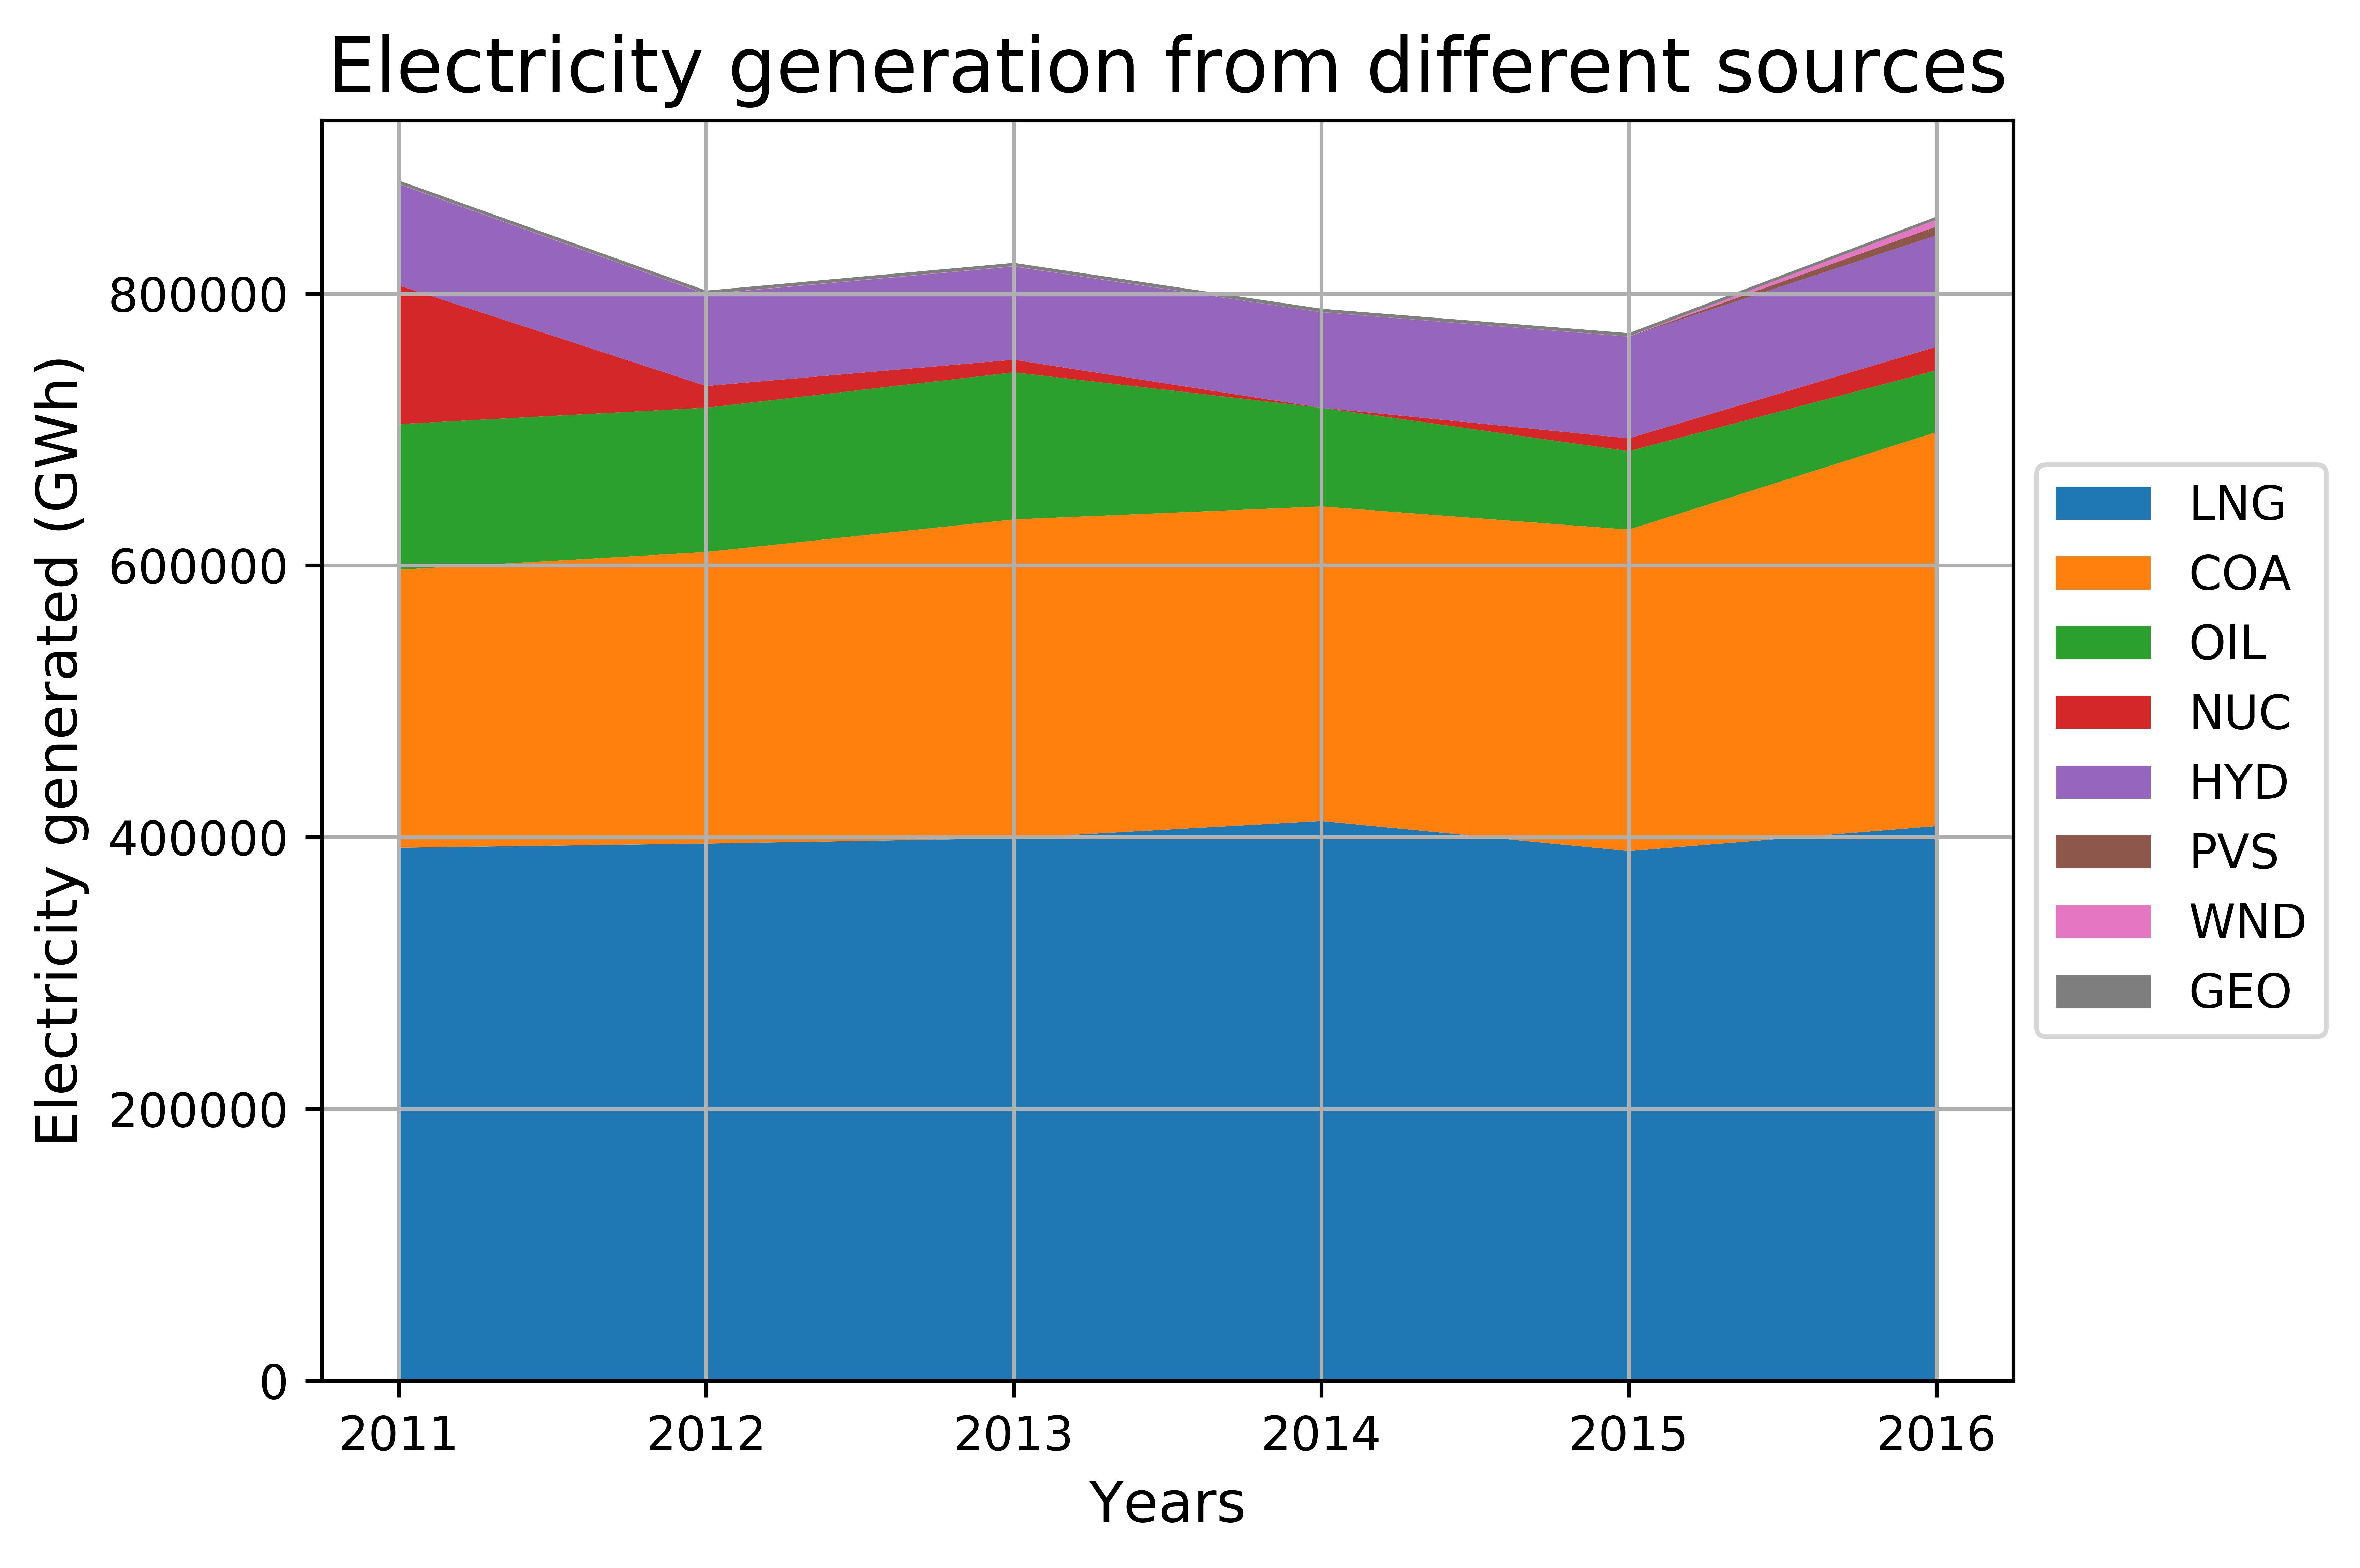
\includegraphics[scale=0.6]{elc-2016}
\caption{Electricity generated from different sources}
\end{figure}

The emitted CO\textsubscript{2} values for the period 2011-16 are as follows. The error is at most 5.7\% \ref{co2err}, which is due to the aforementioned absence of accurate data for 2011, 2012 and 2016. 

\begin{figure}[H]
\centering
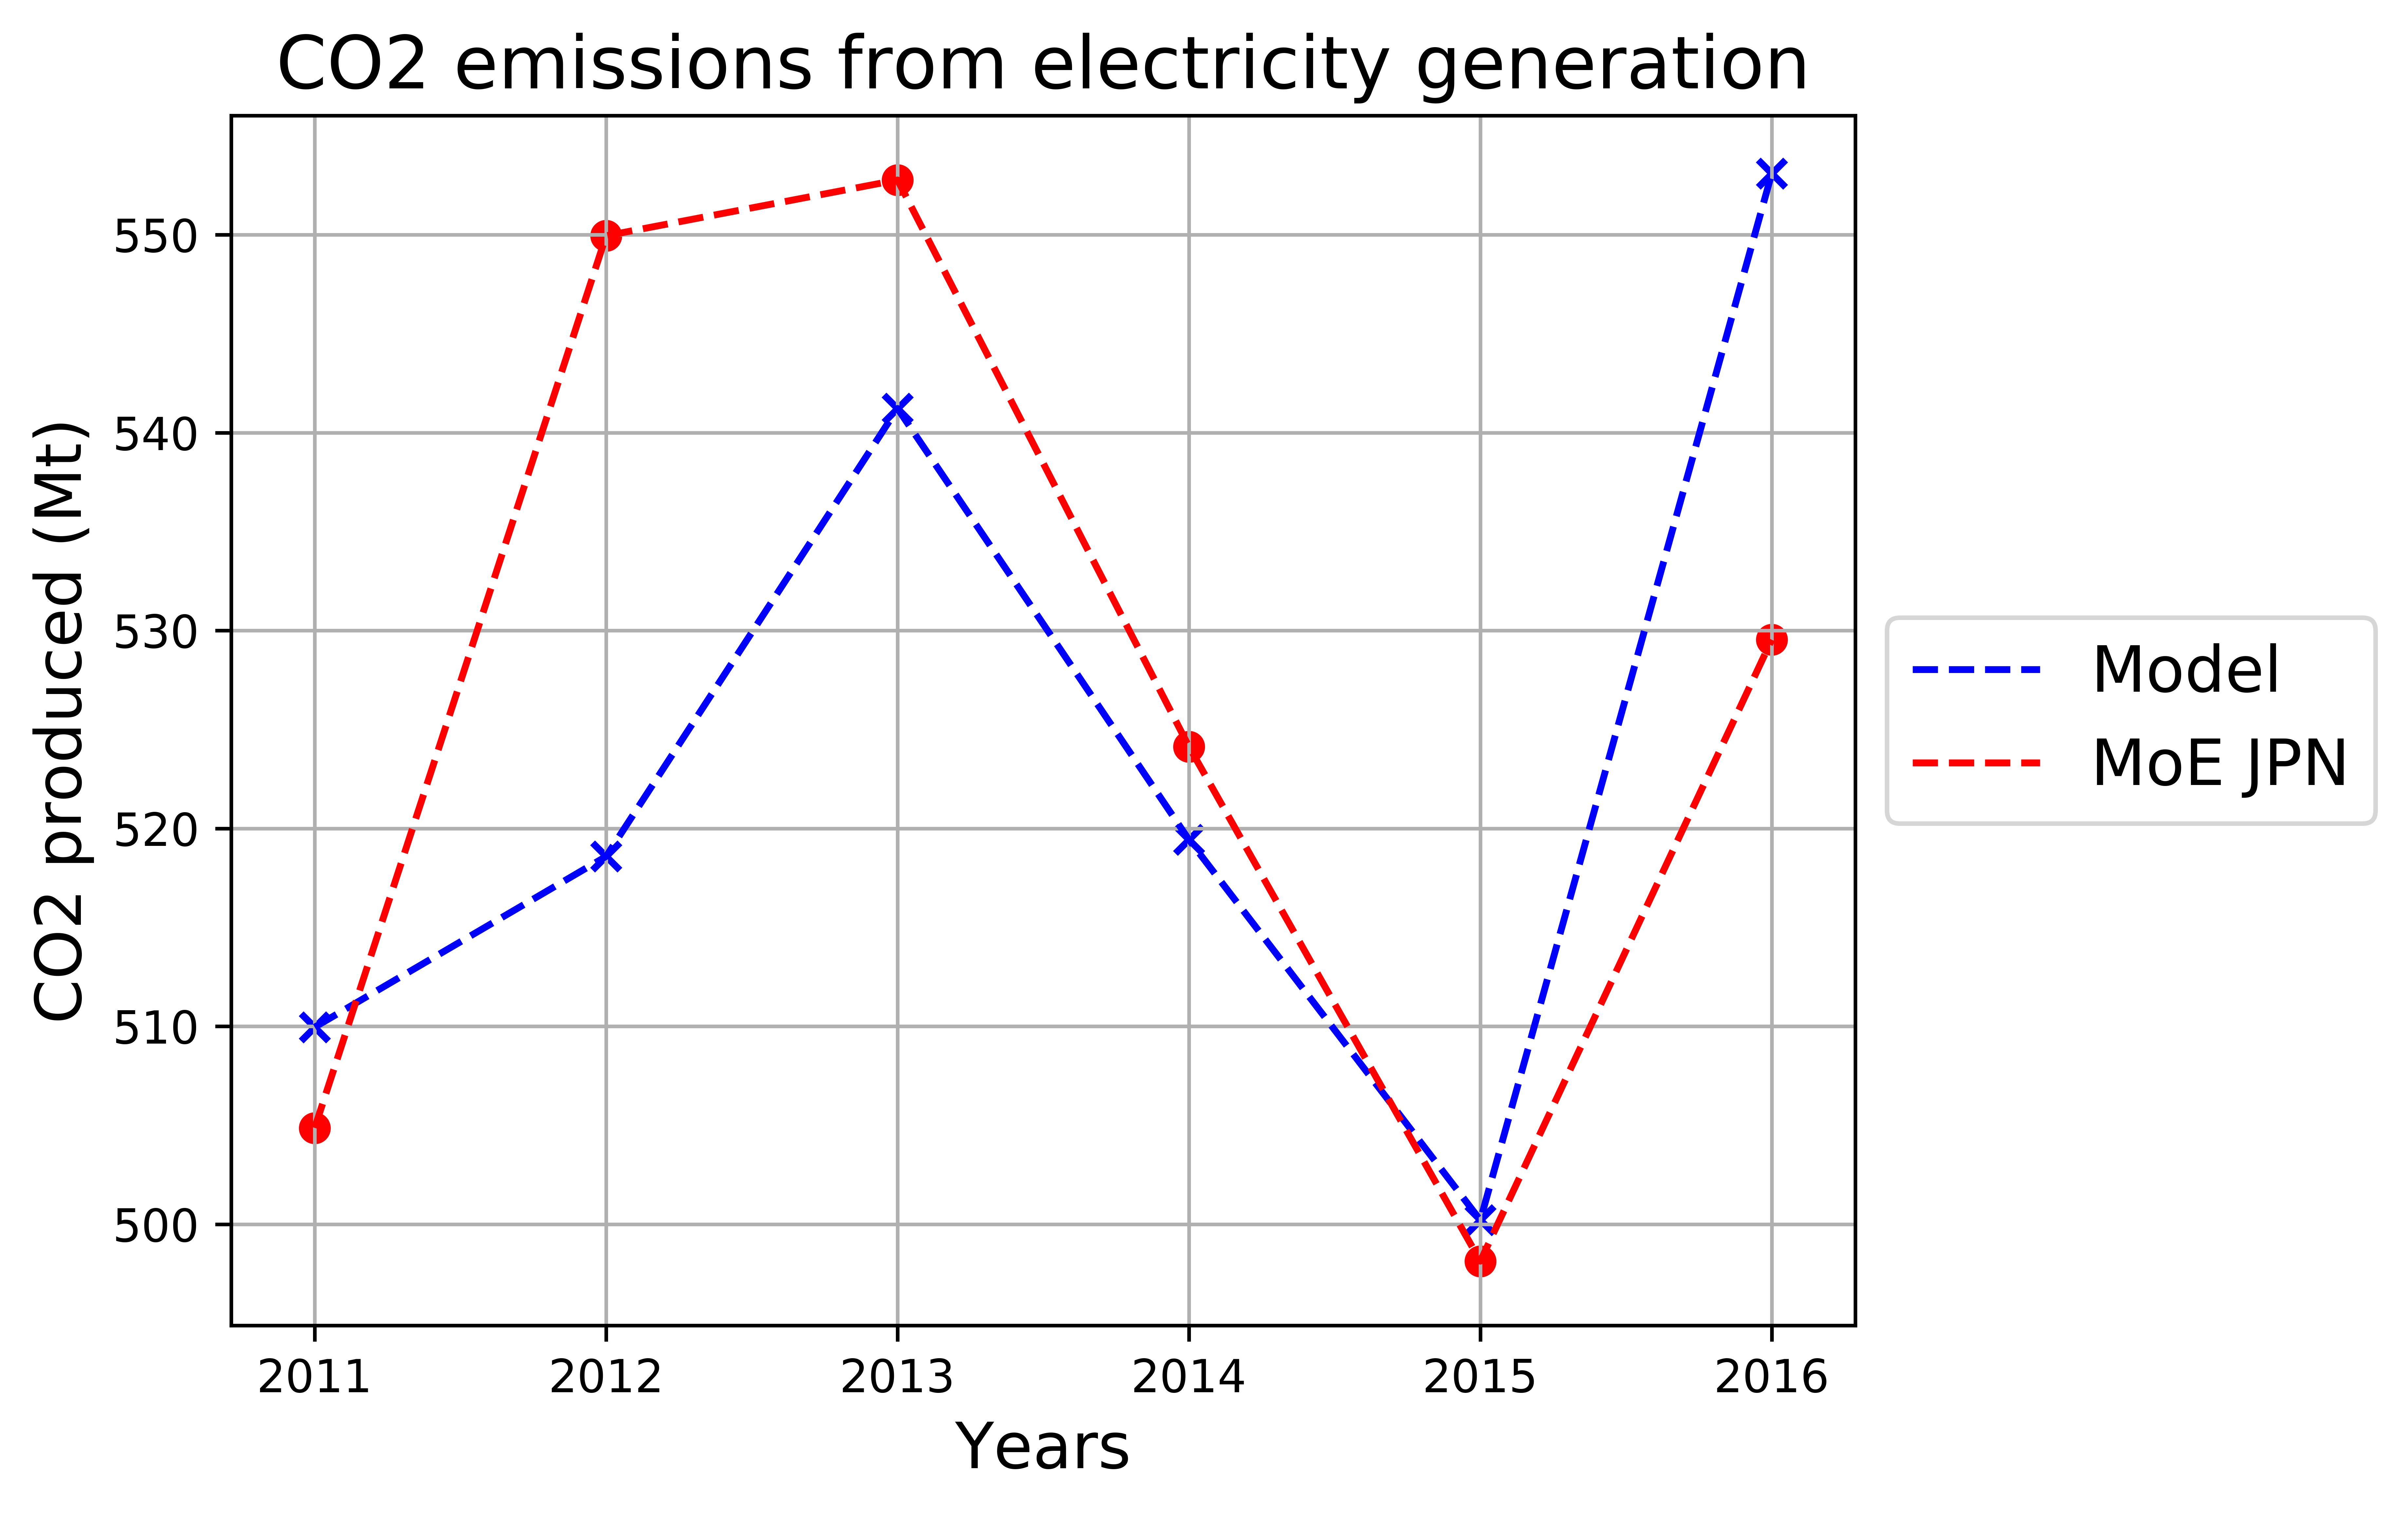
\includegraphics[scale=0.6]{co2-2016}
\caption{CO2 emissions from electricity generation compared with actual emissions reported by Ministry of Environment(MoE), Japan}
\end{figure}

\begin{figure}[H] \label{co2err}
\centering
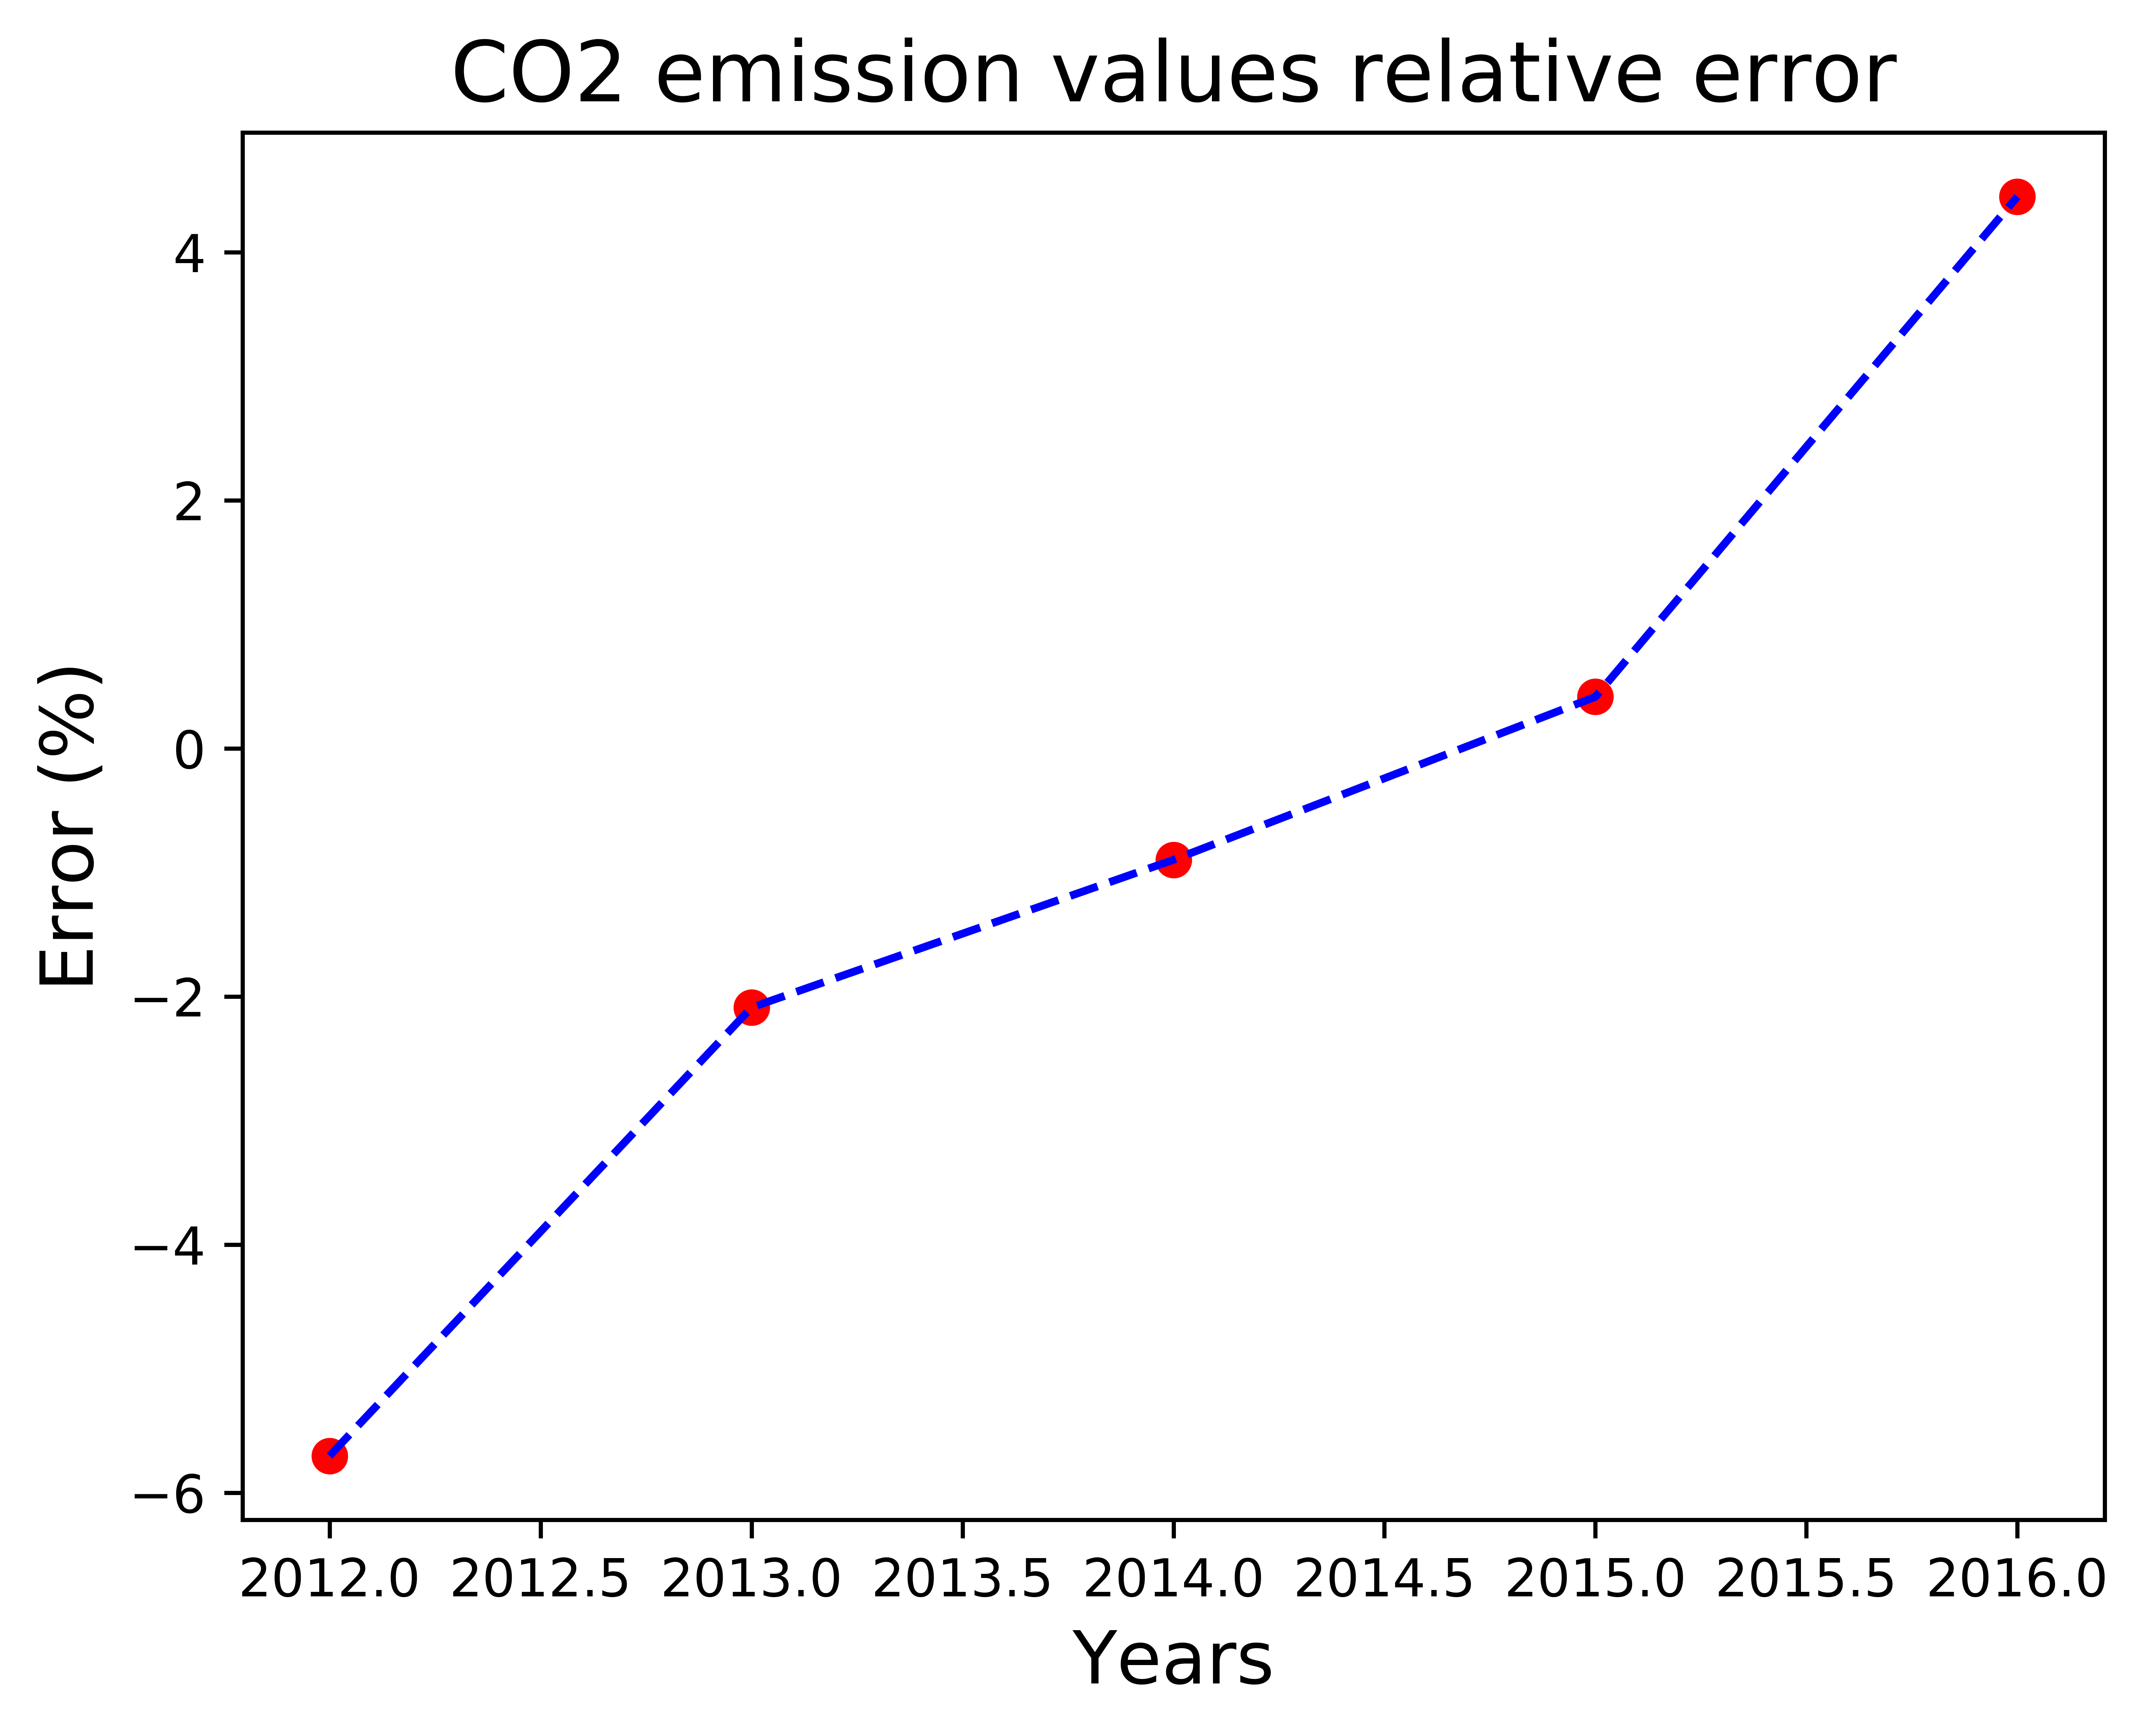
\includegraphics[scale=0.6]{co2-err}
\caption{Relative error in CO2 emissions.}
\end{figure}

\subsection{Post Hoc Analysis and Challenges} 

The project was significantly delayed due to the quality of the documentation and customer support provided by the VEDA developers. The primitive, black-box like nature of the software often produces inexplicable, illogical results and inhibits efficient debugging. Therefore, while data acquisition and organization proceeded at the originally suggested pace, the incorporation of this data into the model has been behind schedule, by about three months. \\

In addition to having incomplete/inaccurate data for 2011, 2012 and 2016, EDMC has been eliminating data related to electricity generation from individual fossil fuels and lumping power from coal, oil, and natural gas into a category called "thermal" in its databank. This complicates the process of estimating CO\textsubscript{2} emissions from these energy sources, since each fossil fuel has a different emission coefficient. Losing the primary data that we have been relying on has affected our pace and the reproducibility of our research significantly. The EDMC databank figures in GWh, instead of in tons of coal or oil, have influenced our model's simplistic design, as discussed previously. Our efforts to find similar data have been unsuccessful. Switching to data in terms of the quantity of raw fossil fuels consumed instead of GWh of electricity produced may require a substantial revision of our model. 

\section{Future Work} 
Considering these challenges, any future efforts on this project will be concentrated in the following areas, in this order of precedence:

\begin{itemize}

\item Acquisition of accurate data for electricity generation from fossil fuels. The most promising source now seems to be the EDMC 2017 handbook.

\item Refining fossil fuel-based electricity generation values and hence CO\textsubscript{2} emission values.

\item Implementation of realistic CO\textsubscript{2} constraints based on Kyoto protocols and I\textsuperscript{2}CNER targets.

\item Refining the demand process and aligning it more closely with realistic projections.

\item Incorporation of I\textsuperscript{2}CNER technologies in the model.

\item Incorporating capacity constraints on technologies such as nuclear power, geothermal power, carbon sequestration etc to model different scenarios.

\item Sensitivity analysis of model parameters to analyze the relative impact of incorporated technologies on the decarbonization goal.

\end{itemize}

In case we must switch to more accurate data that is different from the EDMC figures, we may have to modify the model accordingly. For instance, if the data is in terms of units of fossil fuels consumed, we must model the appropriate fossil fuel conversion processes with the relevant conversion factors and efficiencies. This will further delay the project by another one to two months.


\bibliographystyle{ieeetr}
%\addbibresource{2018-chaube-i2cner-report-sept}
\bibliography{2018-chaube-i2cner-report-sept}

%\bibliographystyle{plain}

%\printbibliography

\end{document}
